%% Be sure to check spelling!

%% Put your name and the proper due date in place

%% Copy the lstinputlisting and figure code as many times as you need
%% Be sure to put in your own file names if appropriate

%% Note that the \includegraphics and \lstinputlisting commands 
%% are currently commented out with %%% - until the
%% files exist, processing this code without them will result in an error
%% so leave the comments until you have created the files!

\documentclass{article}
\usepackage{amsmath}    % loads AMS-Math package
\usepackage{graphicx}   % allows image files
\usepackage{listings}   % allows lstlisting environment
\usepackage[letterpaper, margin=0.5in]{geometry}  % set paper size/margins
\usepackage{EGR103style} % colorful file imports

\begin{document}
\begin{center}
\rule{6.5in}{0.5mm}\\~\\
\textbf{\large EGR 103L -- Fall 2021}\\~\\
\textbf{\huge Lab 5: Structured Programming II}\\~\\
***NAME (NetID)***\\
***Lab Section N, DAY TIMES***\\
***DATE DUE***\\~\\
{\small I understand and have adhered to all the tenets of the Duke Community Standard in completing every part of this assignment.  I understand that a violation of any part of the Standard on any part of this assignment can result in failure of this assignment, failure of this course, and/or suspension from Duke University.} 
\rule{6.5in}{0.5mm}\\
\end{center}
\tableofcontents
\listoffigures
\pagebreak

\section{Chapra 3.4}
\renewcommand{\arraystretch}{1.3}
% Use  \cite{Chapra} and \cite{Other} to give references
% State why you put the cities in the order you did
\begin{center}
\begin{tabular}{ccc}\hline
City & $T_{\mbox{mean}}$ ($^o$C) & $T_{\mbox{peak}}$ ($^o$C) \\ \hline
FIRST CITY & MEAN & PEAK \\
% fill in the rest
LAST CITY & MEAN & PEAK \\ \hline
\end{tabular}
\end{center}
A graph of one years' worth of temperatures for each of the six cities
above is presented in Figure \ref{TempGraph} on page
\pageref{TempGraph}.  The temperatures for each city come from
approximation function given in \cite{Chapra}:
\begin{align*}
% typeset the equation here
\end{align*}

\section{Chapra 4.25}
% Discuss what happens with the different angles

\section{Finding Roots}
% Discuss the different visualizations

\pagebreak
\appendix
\section{Codes}
% Put the name of your file in the subsection name 
% and the listinginput input
% Be sure to include the community standard in codes!
% Add \pagebreaks if they make sense

% Put the files in the same order as the problems; generally, 
% scripts will come first followed by any functions called
% by those scripts.
\lstset{style=python103, language=python} 

\subsection{chapra\_0304.py}
%\lstinputlisting{chapra_0304.py}
\clearpage

\subsection{graph\_temps.py}
%\lstinputlisting{graph_temps.py}
\clearpage

\subsection{cos\_series.py}
%\lstinputlisting{cos_series.py}
\clearpage

\subsection{poly\_root.py}
%\lstinputlisting{poly_root.py}

\clearpage % start Figures on new page

\section{Figures}
\begin{figure}[htb!]
\begin{center}
%\includegraphics{Chapra0304plot.png}
\caption{Yearly temperatures for six cities.\label{TempGraph}}
\end{center}
\end{figure}
\clearpage

\begin{figure}[ht!]
\begin{center}
\begin{tabular}{cc}
%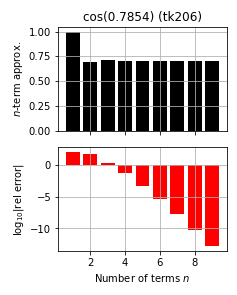
\includegraphics{CosPlot0.png} &
%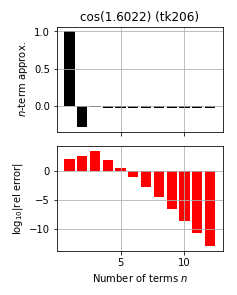
\includegraphics{CosPlot1.png} \\
%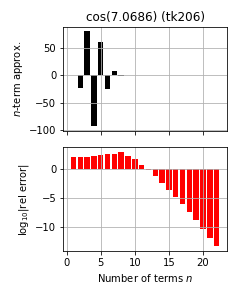
\includegraphics{CosPlot2.png} &
%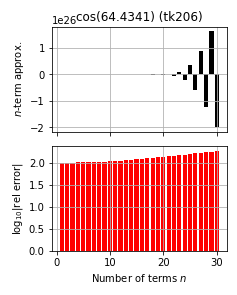
\includegraphics{CosPlot3.png} 
\end{tabular}
\caption{Figures for Cosine Approxmiation}
\end{center}
\end{figure}
\clearpage
\begin{figure}[ht!]
\begin{center}
%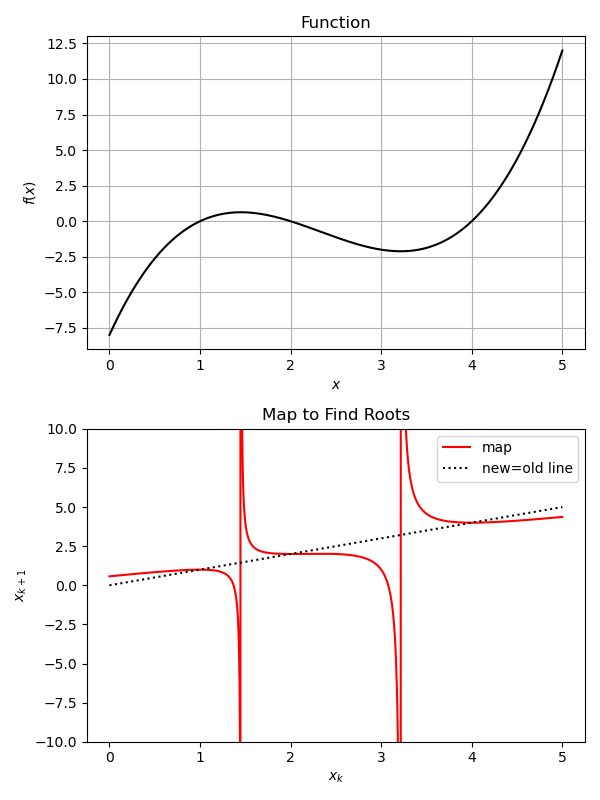
\includegraphics{RootPlot0.png} 
\caption{Function and Derivative}
\end{center}
\end{figure}
\begin{figure}[ht!]
\begin{center}
%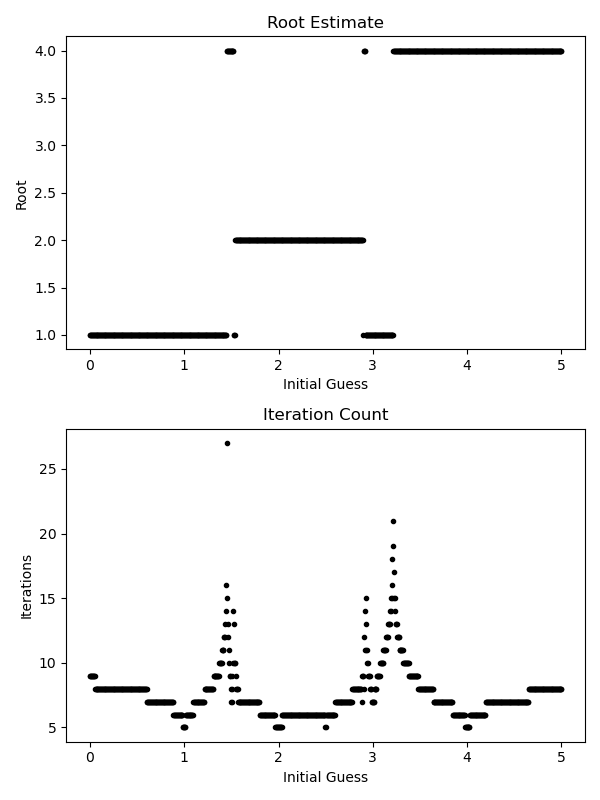
\includegraphics{RootPlot1.png} 
\caption{Root Estimates and Iteration Count}
\end{center}
\end{figure}
\begin{figure}[ht!]
\begin{center}
%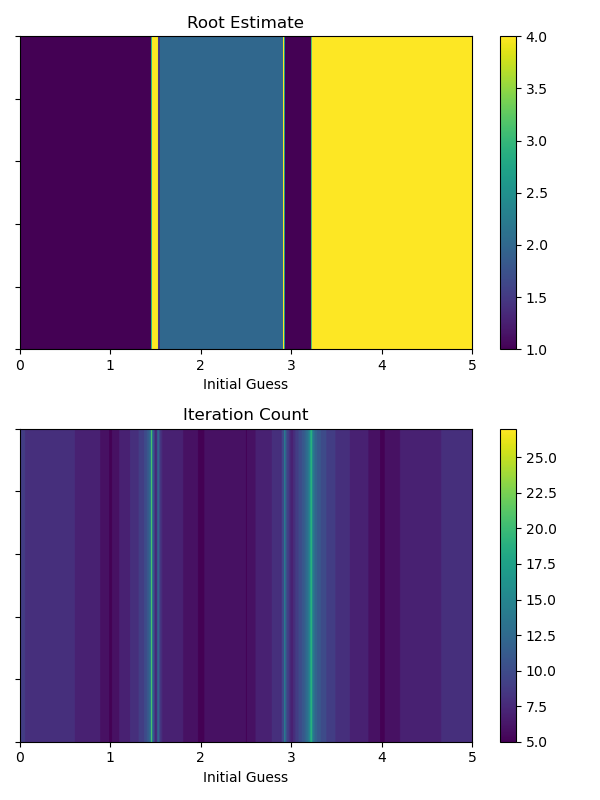
\includegraphics{RootPlot2.png} 
\caption{Root Estimates and Iteration Count - As Image}
\end{center}
\end{figure}
\clearpage

\begin{thebibliography}{9}
\bibitem{Chapra}
  Chapra, Steven C.,
  {\it Applied Numerical Methods with MATLAB for Engineering and Scientists}.
  McGraw-Hill, New York,
  4th Edition,
  2018.
\bibitem{Other}
   Your reference for Durham's mean and peak temperatures
\end{thebibliography}
\end{document}
